\model{Objects}

Consider the definition for a playing card:

\medskip
\begin{javalst}
public class Card {
    private int rank;  // 1=Ace, ..., 11=Jack, 12=Queen, 13=King
    private int suit;  // 0=Clubs, 1=Diamonds, 2=Hearts, 3=Spades

    public Card(int rank, int suit) {
        this.rank = rank;
        this.suit = suit;
    }
}
\end{javalst}

\bigskip
Here is a memory diagram of a \java{Card} object:

\begin{javalst}
    Card card = new Card(8, 1);
\end{javalst}

\vspace{-6.8em}
\hfill 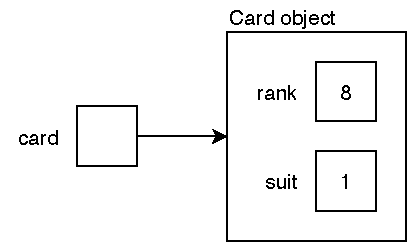
\includegraphics{diagram-object.pdf}
\hspace{4em} \null
\vspace{0.5em}


\quest{15 min}


\Q Which card (i.e., ``the \blank of \blank'') is represented in the diagram?

\begin{answer}[2em]
The 8 of Diamonds.
\end{answer}

\Q In one line of code, show how you would construct the ``4 of Clubs''.

\begin{answer}[2em]
\jans{Card card = new Card(4, 0);}
\end{answer}


\Q What is the difference between lowercase \java{card} and uppercase \java{Card}? Explain in a few sentences how these concepts are illustrated in the diagram.

\begin{answer}[5em]
Lowercase \java{card} is a variable that contains a reference.
Uppercase \java{Card} is a class, from which we create objects.
Variables are small boxes; objects are large boxes that contain variables.
\end{answer}


\Q \label{key2}
How are arrays and objects similar? How are arrays and objects different?
Explain your answer in terms of how they are drawn in memory diagrams.

\begin{answer}[5em]
Both are reference types; their variables have an arrow pointing somewhere else.
Arrays are drawn as contiguous boxes, representing multiple values of the same type.
Objects are drawn as larger boxes, representing multiple variables by name.
\end{answer}


\Q Draw (or describe) a diagram of the following source code:

\begin{javalst}
Card card = null;
\end{javalst}


\begin{answer}[10em]

\includegraphics[scale=1]{card-null.pdf}
\end{answer}


\Q Draw (or describe) a diagram of the following source code:

\begin{javalst}
Card card = new Card(5, 2);
Card copy = card;
\end{javalst}

\begin{answer}[20em]
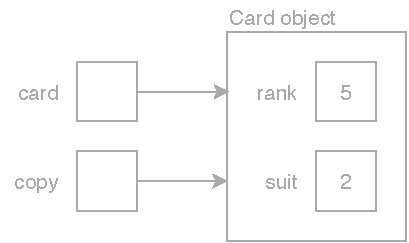
\includegraphics[scale=1]{card-copy.pdf}
\end{answer}


\Q (Optional) Paste the contents of \textit{Card.java} into \href{https://cscircles.cemc.uwaterloo.ca/java_visualize/#code=public+class+ClassNameHere+%7B%0A++++public+static+void+main(String%5B%5D+args)+%7B%0A++++++++%0A++++%7D%0A%7D&mode=edit&showStringsAsObjects=1}{Java Visualizer}.
What differences do you notice between the diagram in Java Visualizer and those in \ref{\currfilename}?

\begin{answer}
Answers might include:
\bull JV says ``Card instance'' instead of ``Card object''.
\bull The object looks like a table, not separate boxes.
\end{answer}
